\documentclass{article}
\usepackage[utf8]{inputenc}
\usepackage{algorithm}
\usepackage{algpseudocode}
\usepackage{braket}
\usepackage{amsmath, amsfonts, amssymb, amsthm}

\newcommand{\norm}[1]{\left\lVert#1\right\rVert}
\algrenewcommand\algorithmicrequire{\textbf{Input:}}
\algrenewcommand\algorithmicensure{\textbf{Output:}}

\makeatletter
\renewcommand{\fnum@algorithm}{\fname@algorithm}
\makeatother



\usepackage{amsfonts}
%\usepackage{braket}
\usepackage[bottom]{footmisc}
\usepackage{xcolor}
\usepackage{amsmath}
\usepackage{enumerate}
\usepackage{tikz}
\usetikzlibrary{matrix,decorations.pathreplacing,quantikz}
\usepackage{mleftright}
\usepackage{amssymb}
\usepackage{mathabx}
\usepackage[margin=20pt]{geometry}

\usetikzlibrary{math}

\begin{document}
\pagestyle{empty}



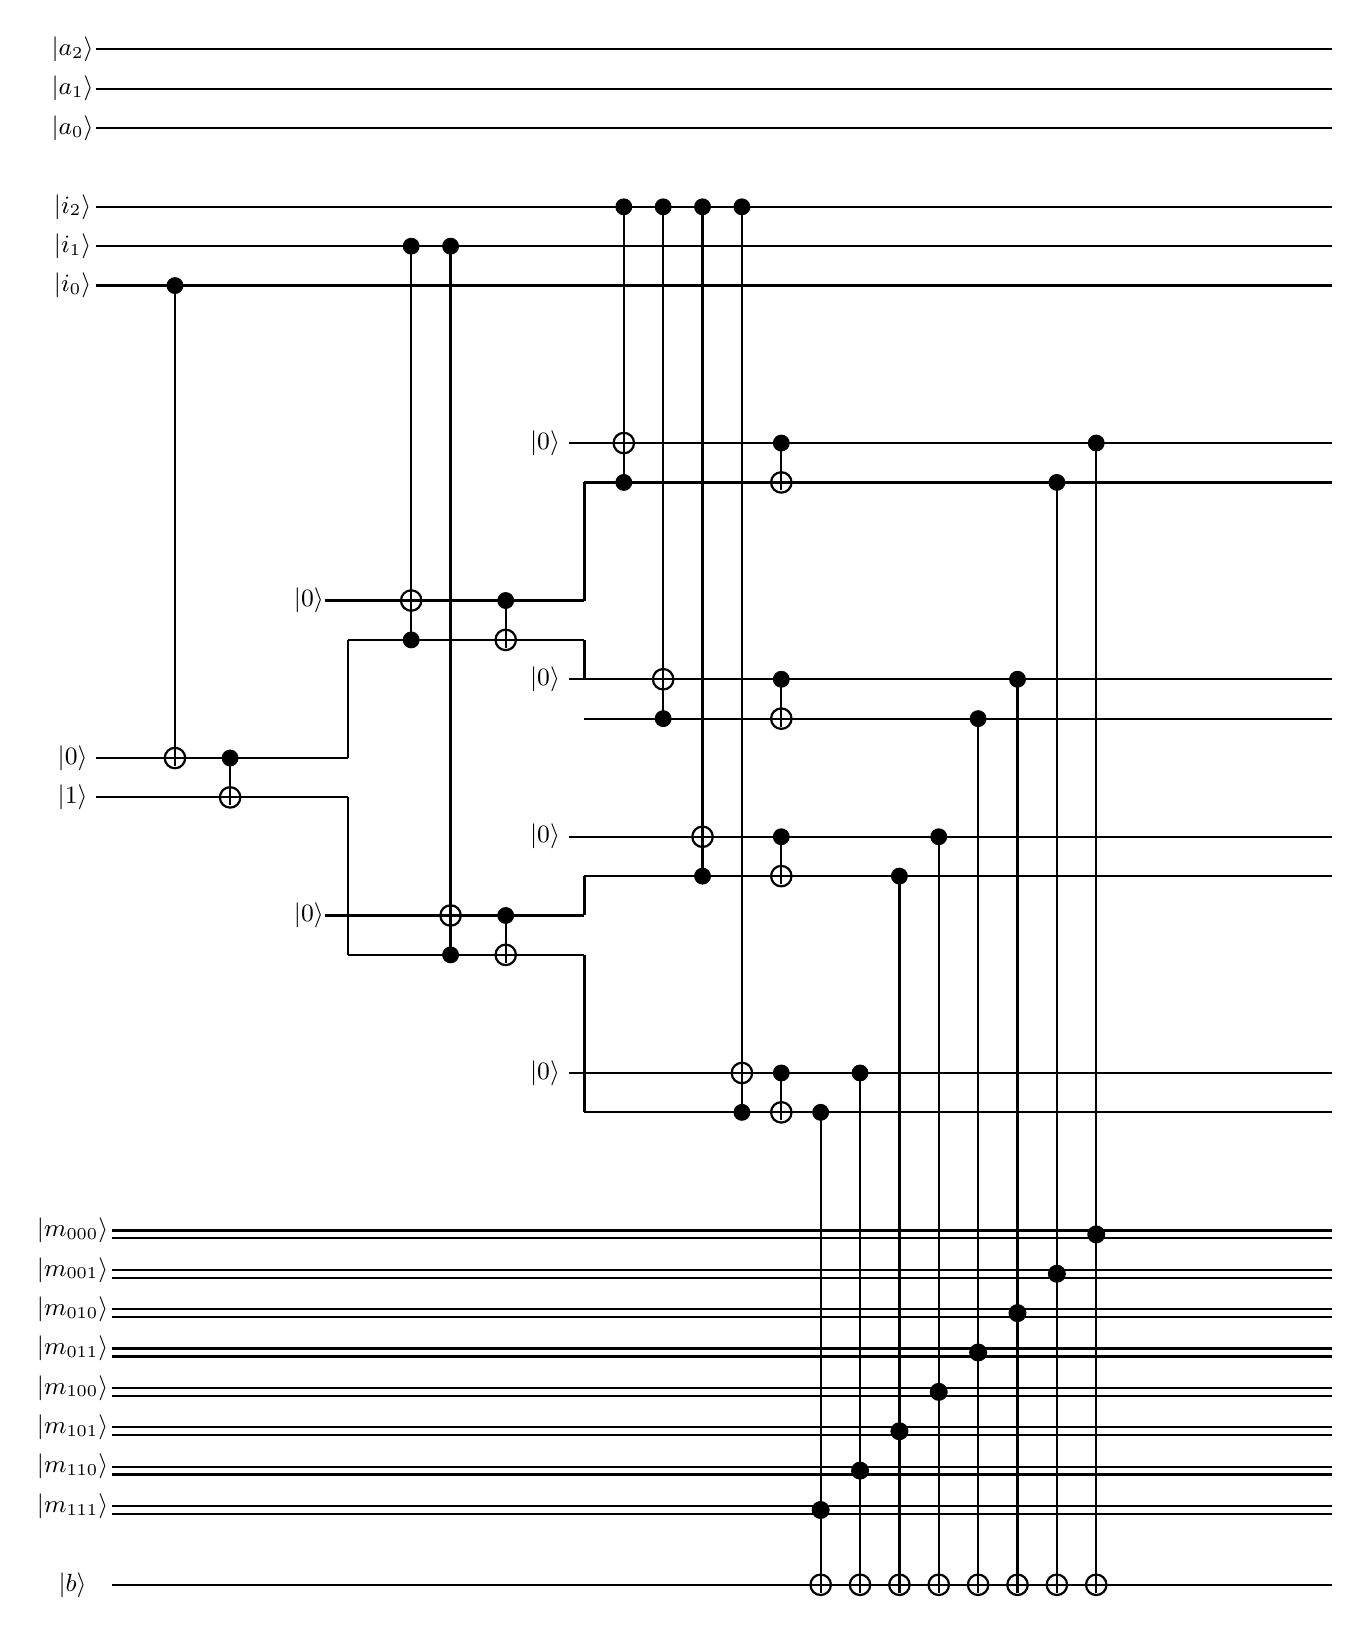
\begin{tikzpicture}
    % address register
    \draw (0, 0) node{\small $\ket{i_0}$};
    \draw (0, 0.5) node{\small $\ket{i_1}$};
    \draw (0, 1) node{\small $\ket{i_2}$};

    % memory register
    \draw (0, -12) node{\small $\ket{m_{000}}$};
    \draw (0, -12.5) node{\small $\ket{m_{001}}$};
    \draw (0, -13) node{\small $\ket{m_{010}}$};
    \draw (0, -13.5) node{\small $\ket{m_{011}}$};
    \draw (0, -14) node{\small $\ket{m_{100}}$};
    \draw (0, -14.5) node{\small $\ket{m_{101}}$};
    \draw (0, -15) node{\small $\ket{m_{110}}$};
    \draw (0, -15.5) node{\small $\ket{m_{111}}$};

    % ancilla qubits register
    \draw (0, 2) node{\small $\ket{a_0}$};
    \draw (0, 2.5) node{\small $\ket{a_1}$};
    \draw (0, 3) node{\small $\ket{a_2}$};
    

    % target register 
    \draw (0, -16.5) node{\small $\ket{b}$};

    % horizontal line ancilla register
    \draw [-] [thick] (0+0.3, 2) to (16, 2);
    \draw [-] [thick] (0+0.3, 2.5) to (16, 2.5);
    \draw [-] [thick] (0+0.3, 3) to (16, 3);

    % horizontal lines address register
    \draw [-] [thick] (0+0.3, 0) to (16, 0);
    \draw [-] [thick] (0+0.3, 0.5) to (16, 0.5);
    \draw [-] [thick] (0+0.3, 1) to (16, 1);

    % horizontali lines memory and target 
    \draw [-] [thick] (0+0.5, -12-0.1) to (16, -12-0.1);
  \draw [-] [thick] (0+0.5, -12.5-0.1) to (16, -12.5-0.1);
  \draw [-] [thick] (0+0.5, -13-0.1) to (16, -13-0.1);
   \draw [-] [thick] (0+0.5, -13.5-0.1) to (16, -13.5-0.1);
   \draw [-] [thick] (0+0.5, -14-0.1) to (16, -14-0.1);
   \draw [-] [thick] (0+0.5, -14.5-0.1) to (16, -14.5-0.1);
   \draw [-] [thick] (0+0.5, -15.5-0.1) to (16, -15.5-0.1);
   \draw [-] [thick] (0+0.5, -15-0.1) to (16, -15-0.1);

  \draw [-] [thick] (0+0.5, -16.5) to (16, -16.5);


    % double lines for classical memory register
      \draw [-] [thick] (0+0.5, -12) to (16, -12);
  \draw [-] [thick] (0+0.5, -12.5) to (16, -12.5);
  \draw [-] [thick] (0+0.5, -13) to (16, -13);
   \draw [-] [thick] (0+0.5, -13.5) to (16, -13.5);
   \draw [-] [thick] (0+0.5, -14) to (16, -14);
   \draw [-] [thick] (0+0.5, -14.5) to (16, -14.5);
   \draw [-] [thick] (0+0.5, -15.5) to (16, -15.5);
   \draw [-] [thick] (0+0.5, -15) to (16, -15);
  \draw [-] [thick] (0+0.5, -16.5) to (16, -16.5);



    % ANCILLA REGISTERS
    % central ancilla register
    \draw (0, -6) node{\small $\ket{0}$};
    \draw (0, -6.5) node{\small $\ket{1}$};

    % above and below angilla register pt 2
    \draw (3, -4) node{\small $\ket{0}$};
    %\draw (3, -4.5) node{\small $\ket{1}$};

    \draw (3, -8) node{\small $\ket{0}$};
    %\draw (3, -8.5) node{\small $\ket{1}$};


    % above and below kets pt 3
    \draw (6, -2) node{\small $\ket{0}$};
    %\draw (6, -2.5) node{\small $\ket{1}$};

    \draw (6, -10) node{\small $\ket{0}$};
    %\draw (6, -10.5) node{\small $\ket{1}$};

    \draw (6, -5) node{\small $\ket{0}$};
    %\draw (6, -5.5) node{\small $\ket{1}$};

    \draw (6, -7) node{\small $\ket{0}$};
    %\draw (6, -7.5) node{\small $\ket{1}$};



    % horizontal lines 2nd level of ancillas
    \draw [-] [thick] (0+0.3, -6) to (3+0.5, -6);   % 0 
    \draw [-] [thick] (0+0.3, -6.5) to (3+0.5, -6.5);  % 1


    % % horizontal lines pt 2
    \draw [-] [thick] (3+0.5, -4.5) to (3+3.5, -4.5);   % 1
    \draw [-] [thick] (3+0.5, -8.5) to (3+3.5, -8.5);   % 1
    
    \draw [-] [thick] (3+0.2, -4) to (3+3.5, -4);   % 0
    \draw [-] [thick] (3+0.2, -8) to (3+3.5, -8);   % 0


    % % horizontal lines pt 3 
    \draw [-] [thick] (6+0.5-0.2, -2) to (16, -2);   % 0
    \draw [-] [thick] (6+0.5, -2.5) to (16, -2.5);   % 1

    \draw [-] [thick] (6+0.5-0.2, -5) to (16, -5);   % 0
    \draw [-] [thick] (6+0.5, -5.5) to (16, -5.5);   % 1

    \draw [-] [thick] (6+0.5-0.2, -7) to (16, -7);   % 0
    \draw [-] [thick] (6+0.5, -7.5) to (16, -7.5);   % 1

    \draw [-] [thick] (6+0.5-0.2, -10) to (16, -10);   % 0
    \draw [-] [thick] (6+0.5, -10.5) to (16, -10.5);   % 1

    
    % vertical lines (central to external)
    \draw [-] [thick] (3+0.5, -6) to (3+0.5, -4.5); % 0 -> 1
    \draw [-] [thick] (3+0.5, -6.5) to (3+0.5, -8.5); 

    \draw [-] [thick] (6+0.5, -4) to (6+0.5, -2.5);
    \draw [-] [thick] (6+0.5, -4.5) to (6+0.5, -5);
    \draw [-] [thick] (6+0.5, -8.5) to (6+0.5, -10.5);   % 4th
    \draw [-] [thick] (6+0.5, -8) to (6+0.5, -7.5);




     % CNOTS
     \draw[fill=black] (0+0.3+1, 0) circle [radius=0.1];
     \draw (0+0.3+1, -6) [thick] circle (0.13);
     \draw [-] [thick] (0+0.3+1, 0) to (0+0.3+1, -6);
     \draw [-] [thick] (0+0.3+1, -6-0.1) to (0+0.3+1, -6+0.1);

    \draw[fill=black] (2, -6) circle [radius=0.1];
     \draw (2, -6.5) [thick] circle (0.13);
     \draw [-] [thick] (2, -6) to (2, -6.5);
     \draw [-] [thick] (2, -6.5+0.1) to (2, -6.5-0.1);


    \draw[fill=black] (3+0.3+1, 0.5) circle [radius=0.1];
   \draw (3+0.3+1, -4) [thick] circle (0.13);
   \draw [-] [thick] (3+0.3+1, 0.5) to (3+0.3+1, -4);
   \draw [-] [thick] (3+0.3+1, -4.5) to (3+0.3+1, -4);
    \draw[fill=black] (3+0.3+1, -4.5) circle [radius=0.1];

    \draw[fill=black] (3+0.3+1+0.5, 0.5) circle [radius=0.1];
    \draw (3+0.3+1+0.5, -8) [thick] circle (0.13);
    \draw [-] [thick] (3+0.3+1+0.5, 0.5) to (3+0.3+1+0.5, -8.5);
    \draw [-] [thick] (3+0.3+1+0.5, -4.5) to (3+0.3+1+0.5, -4);
    \draw[fill=black] (3+0.3+1+0.5, -8.5) circle [radius=0.1];

    \draw[fill=black] (5.5, -4) circle [radius=0.1];
     \draw (5.5, -4.5) [thick] circle (0.13);
     \draw [-] [thick] (5.5, -4) to (5.5, -4.5);
     \draw [-] [thick] (5.5, -4.5+0.1) to (5.5, -4.5-0.1);

    \draw[fill=black] (5.5, -8) circle [radius=0.1];
     \draw (5.5, -8.5) [thick] circle (0.13);
     \draw [-] [thick] (5.5, -8) to (5.5, -8.5);
     \draw [-] [thick] (5.5, -8.5+0.1) to (5.5, -8.5-0.1);


    % last controlled on index register
    \draw[fill=black] (7, 1) circle [radius=0.1];
    \draw[fill=black] (7, -2.5) circle [radius=0.1];
    \draw (7, -2) [thick] circle (0.13);
     \draw [-] [thick] (7, -2.5) to (7, 1);



    \draw[fill=black] (7.5, 1) circle [radius=0.1];
    \draw[fill=black] (7.5, -5.5) circle [radius=0.1];
    \draw (7.5, -5) [thick] circle (0.13);
     \draw [-] [thick] (7.5, -5.5) to (7.5, 1);


    \draw[fill=black] (8, 1) circle [radius=0.1];
    \draw[fill=black] (8, -7.5) circle [radius=0.1];
    \draw (8, -7) [thick] circle (0.13);
     \draw [-] [thick] (8, -7.5) to (8, 1);

     
    \draw[fill=black] (8.5, 1) circle [radius=0.1];
    \draw[fill=black] (8.5, -10.5) circle [radius=0.1];
    \draw (8.5, -10) [thick] circle (0.13);
     \draw [-] [thick] (8.5, -10.5) to (8.5, 1);


     % last layer of cnots
    % \draw[fill=black] (8.5, -2) circle [radius=0.1];
    \draw[fill=black] (9, -2) circle [radius=0.1];
    \draw (9, -2.5) [thick] circle (0.13);
    \draw [-] [thick] (9, -2.5-0.1) to (9, -2);
     
    \draw[fill=black] (9, -5) circle [radius=0.1];
    \draw (9, -5.5) [thick] circle (0.13);
    \draw [-] [thick] (9, -5.5-0.1) to (9, -5);


    \draw[fill=black] (9, -7) circle [radius=0.1];
    \draw (9, -7.5) [thick] circle (0.13);
    \draw [-] [thick] (9, -7.5-0.1) to (9, -7);

    \draw[fill=black] (9, -10) circle [radius=0.1];
    \draw (9, -10.5) [thick] circle (0.13);
    \draw [-] [thick] (9, -10.5-0.1) to (9, -10);

    % writing in memory
    \draw[fill=black] (9.5, -10.5) circle [radius=0.1];
    \draw[fill=black] (9.5, -15.5-0.05) [thick] circle (0.1);
    \draw (9.5, -16.5) [thick] circle (0.13);
    \draw [-] [thick] (9.5, -10.5) to (9.5, -16.5-0.1);

    \draw[fill=black] (10, -10) circle [radius=0.1];
    \draw[fill=black] (10, -15-0.05) [thick] circle (0.1);
    \draw (10, -16.5) [thick] circle (0.13);
    \draw [-] [thick] (10, -10) to (10, -16.5-0.1);

    \draw[fill=black] (10.5, -7.5) circle [radius=0.1];
    \draw[fill=black] (10.5, -14.5-0.05) [thick] circle (0.1);
    \draw (10.5, -16.5) [thick] circle (0.13);
    \draw [-] [thick] (10.5, -7.5) to (10.5, -16.5-0.1);

    \draw[fill=black] (11, -7) circle [radius=0.1];
    \draw[fill=black] (11, -14-0.05) [thick] circle (0.1);
    \draw (11, -16.5) [thick] circle (0.13);
    \draw [-] [thick] (11, -7) to (11, -16.5-0.1);


    \draw[fill=black] (11.5, -5.5) circle [radius=0.1];
    \draw[fill=black] (11.5, -13.5-0.05) [thick] circle (0.1);
    \draw (11.5, -16.5) [thick] circle (0.13);
    \draw [-] [thick] (11.5, -5.5) to (11.5, -16.5-0.1);

    \draw[fill=black] (12, -5) circle [radius=0.1];
    \draw[fill=black] (12, -13-0.05) [thick] circle (0.1);
    \draw (12, -16.5) [thick] circle (0.13);
    \draw [-] [thick] (12, -5) to (12, -16.5-0.1);


    \draw[fill=black] (12.5, -2.5) circle [radius=0.1];
    \draw[fill=black] (12.5, -12.5-0.05) [thick] circle (0.1);
    \draw (12.5, -16.5) [thick] circle (0.13);
    \draw [-] [thick] (12.5, -2.5) to (12.5, -16.5-0.1);

    \draw[fill=black] (13, -2) circle [radius=0.1];
    \draw[fill=black] (13, -12-0.05) [thick] circle (0.1);
    \draw (13, -16.5) [thick] circle (0.13);
    \draw [-] [thick] (13, -2) to (13, -16.5-0.1);
     

\end{tikzpicture}





\end{document}
